% !TeX spellcheck = en_GB
% !TEX program = xelatex+makeindex+bibtex
% !TeX TXS-program:pdflatex = txs:///xelatex %
\documentclass[final,a4paper]{report} %scrreprt of scrartcl
%!TEX program=xelatex+makeindex+bibtex
% Include all project wide packages here.
\usepackage{fullpage}
\usepackage{polyglossia}
\setmainlanguage{english}
\usepackage{csquotes}
\usepackage{graphicx}
\usepackage{epstopdf}
\usepackage{pdfpages}
\usepackage{caption}
\usepackage[list=true]{subcaption}
\usepackage{float}
\usepackage{standalone}
\usepackage{import}
\usepackage{tocloft}
\usepackage{wrapfig}
\usepackage{authblk}
\usepackage{array}
\usepackage{booktabs}
\usepackage[toc,page,title,titletoc]{appendix}
\usepackage{xunicode}
\usepackage{fontspec}
\usepackage{pgfplots}
\usepackage{SIunitx}
\usepackage{units}
\pgfplotsset{compat=newest}
\pgfplotsset{plot coordinates/math parser=false}
\newlength\figureheight 
\newlength\figurewidth
\usepackage{amsmath}
\usepackage{mathtools}
\usepackage{unicode-math}
\usepackage{rotating}
\usepackage{fancyhdr}
\usepackage{titlesec}
\usepackage{blindtext}
\usepackage{color}
\usepackage[margin=3.5cm,headheight=35pt]{geometry}
\usepackage[
    backend=bibtexu,
	texencoding=utf8,
bibencoding=utf8,
    style=ieee,
    sortlocale=en_US,
    language=auto
]{biblatex}
\usepackage{listings}
\usepackage{wrapfig}
\newcommand{\includecode}[4][c]{\lstinputlisting[caption=#2, escapechar=, style=#1,label=#4]{#3}}
\newcommand{\superscript}[1]{\ensuremath{^{\textrm{#1}}}}
\newcommand{\subscript}[1]{\ensuremath{_{\textrm{#1}}}}


\newcommand{\chapternumber}{\thechapter}
\renewcommand{\appendixname}{Appendix}
\renewcommand{\appendixtocname}{Appendices}
\renewcommand{\appendixpagename}{Appendices}

\usepackage[hidelinks]{hyperref} %<--------ALTIJD ALS LAATSTE

%!TEX program=xelatex+makeindex+bibtex
\renewcommand{\familydefault}{\sfdefault}

\setmainfont[Ligatures=TeX]{Calibri}
\setmathfont{Asana Math}
\setmonofont{Lucida Console}

%\definecolor{chapterbarcolor}{cmyk}{.52,.32,0,0}
%\definecolor{footrulecolor}{cmyk}{.52,.32,0,0}

\definecolor{chapterbarcolor}{gray}{0.75}
\definecolor{footrulecolor}{gray}{0.75}

\fancypagestyle{plain}{%
  \fancyhf{}    
  \fancyfoot[L]{\ifnum\value{chapter}>0 \chaptername\ \thechapter. \fi}
  \fancyfoot[C]{\thepage}
  \fancyfoot[R]{\small \today}
  \renewcommand{\headrulewidth}{0pt}
  \renewcommand{\footrulewidth}{2pt}
  \renewcommand{\footrule}{\hbox to\headwidth{%
  \color{footrulecolor}\leaders\hrule height \footrulewidth\hfill}}
}

\pagestyle{plain}

\newcommand{\hsp}{\hspace{20pt}}
\titleformat{\chapter}[hang]{\Huge\bfseries}{\chapternumber\hsp\textcolor{chapterbarcolor}{|}\hsp}{0pt}{\Huge\bfseries}
\titlespacing{\chapter}{0pt}{0pt}{1pt}
\renewcommand{\familydefault}{\sfdefault}
\renewcommand{\arraystretch}{1.2}
\setlength{\headheight}{0pt} 
\setlength\parindent{0pt}
\setlength{\parskip}{0.3cm plus4mm minus3mm}
\setlength\cftaftertoctitleskip{5pt}
\setlength\cftbeforetoctitleskip{20pt}

%For code listings
\definecolor{black}{rgb}{0,0,0}
\definecolor{browntags}{rgb}{0.65,0.1,0.1}
\definecolor{bluestrings}{rgb}{0,0,1}
\definecolor{graycomments}{rgb}{0.4,0.4,0.4}
\definecolor{redkeywords}{rgb}{1,0,0}
\definecolor{bluekeywords}{rgb}{0.13,0.13,0.8}
\definecolor{greencomments}{rgb}{0,0.5,0}
\definecolor{redstrings}{rgb}{0.9,0,0}
\definecolor{purpleidentifiers}{rgb}{0.01,0,0.01}


\lstdefinestyle{csharp}{
language=[Sharp]C,
showspaces=false,
showtabs=false,
breaklines=true,
showstringspaces=false,
breakatwhitespace=true,
escapeinside={(*@}{@*)},
columns=fullflexible,
commentstyle=\color{greencomments},
keywordstyle=\color{bluekeywords}\bfseries,
stringstyle=\color{redstrings},
identifierstyle=\color{purpleidentifiers},
basicstyle=\ttfamily\small}

\lstdefinestyle{c}{
language=C,
showspaces=false,
showtabs=false,
breaklines=true,
showstringspaces=false,
breakatwhitespace=true,
escapeinside={(*@}{@*)},
columns=fullflexible,
commentstyle=\color{greencomments},
keywordstyle=\color{bluekeywords}\bfseries,
stringstyle=\color{redstrings},
identifierstyle=\color{purpleidentifiers},
}

\lstdefinestyle{matlab}{
language=Matlab,
showspaces=false,
showtabs=false,
breaklines=true,
showstringspaces=false,
breakatwhitespace=true,
escapeinside={(*@}{@*)},
columns=fullflexible,
commentstyle=\color{greencomments},
keywordstyle=\color{bluekeywords}\bfseries,
stringstyle=\color{redstrings},
identifierstyle=\color{purpleidentifiers}
}

\lstdefinestyle{vhdl}{
language=VHDL,
showspaces=false,
showtabs=false,
breaklines=true,
showstringspaces=false,
breakatwhitespace=true,
escapeinside={(*@}{@*)},
columns=fullflexible,
commentstyle=\color{greencomments},
keywordstyle=\color{bluekeywords}\bfseries,
stringstyle=\color{redstrings},
identifierstyle=\color{purpleidentifiers}
}

\lstdefinestyle{xaml}{
language=XML,
showspaces=false,
showtabs=false,
breaklines=true,
showstringspaces=false,
breakatwhitespace=true,
escapeinside={(*@}{@*)},
columns=fullflexible,
commentstyle=\color{greencomments},
keywordstyle=\color{redkeywords},
stringstyle=\color{bluestrings},
tagstyle=\color{browntags},
morestring=[b]",
  morecomment=[s]{<?}{?>},
  morekeywords={xmlns,version,typex:AsyncRecords,x:Arguments,x:Boolean,x:Byte,x:Char,x:Class,x:ClassAttributes,x:ClassModifier,x:Code,x:ConnectionId,x:Decimal,x:Double,x:FactoryMethod,x:FieldModifier,x:Int16,x:Int32,x:Int64,x:Key,x:Members,x:Name,x:Object,x:Property,x:Shared,x:Single,x:String,x:Subclass,x:SynchronousMode,x:TimeSpan,x:TypeArguments,x:Uid,x:Uri,x:XData,Grid.Column,Grid.ColumnSpan,Click,ClipToBounds,Content,DropDownOpened,FontSize,Foreground,Header,Height,HorizontalAlignment,HorizontalContentAlignment,IsCancel,IsDefault,IsEnabled,IsSelected,Margin,MinHeight,MinWidth,Padding,SnapsToDevicePixels,Target,TextWrapping,Title,VerticalAlignment,VerticalContentAlignment,Width,WindowStartupLocation,Binding,Mode,OneWay,xmlns:x}
}

%defaults
\lstset{
basicstyle=\ttfamily\scriptsize ,
extendedchars=false,
numbers=left,
numberstyle=\ttfamily\tiny,
stepnumber=1,
tabsize=4,
numbersep=5pt
}
\addbibresource{../../library/bibliography.bib}
\author{Fairphone Repair Group}
\title{Fairphone Repairability}
\date{\today}
\begin{document}
	\chapter{Packaging}
	\label{ch:packaging}
	Nowadays, all phones are delivered in their luxurious packages which unfortunately serve no purpose after the delivery. Usually, they are either thrown away (hopefully through recycling) or left forgotten in a drawer or closet to be found again years later to be disposed. The team thought that this element had a lot of room for improvement, and started to think about a way to make the packaging useful even after delivery. The idea came to use it in the process of repairing, facilitating the DIY experience of the user. 
	
	The first packaging design was inspired by a repair mat. A repair mat is divided into several sections which can each hold different specific components for an better visual organisation. Keeping everything as simple as possible and providing the means to easily repair a phone are the key elements to improving the DIY repair experience of the user. To incorporate this idea into the packaging, a design was created which can be seen in figure \ref{fig:Box design 1}. The purpose of the slots is to use them as trays to know exactly what component/module/screw goes where and in what order it was taken apart. 
	
	As an important note, the sketch presented is not accurate. It is in fact not even designed to the Fairphone 2 since the order of disassembly of the modules is unknown, just like the size of every module. The sketch serves purely as a visual aid of what the team intends to achieve.
	
	\begin{figure}[H]
		\centering
		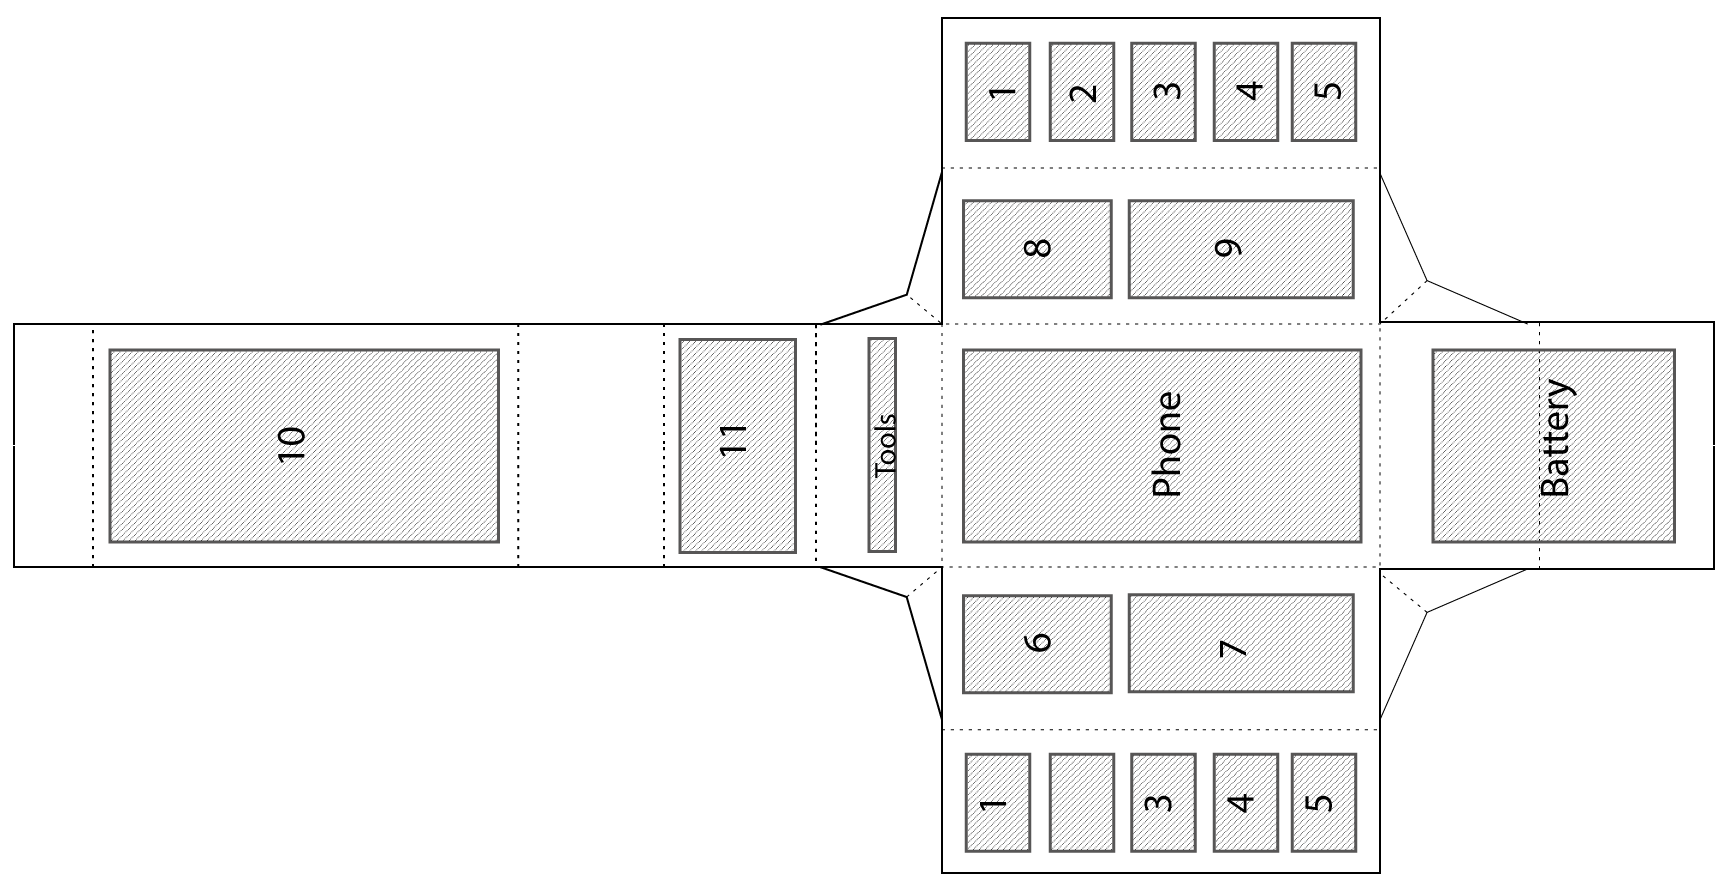
\includegraphics[width=0.8\textwidth]{resources/BoxDesign1}
		\caption{The first re-design of the Fairphone 2 packaging}
		\label{fig:Box design 1}
	\end{figure}
	
	When the first design was brought to life through a prototype, it was clear pretty quickly that it wasn't the right way to go. In fact, it proved to be a very weak structure layout and would not be able to protect the phone during shipment, or even promise to last longer than a few repair sessions. The weakness of the box was mostly due all the parts that were folded and taped together. The first prototype can be seen in figure \ref{fig:Prototype of box design 1}. To make this more complex design stronger, stiffer and more polluting materials would be required, compromising Fairphones awareness-raising image.
	
	\begin{figure}[H]
		\centering
		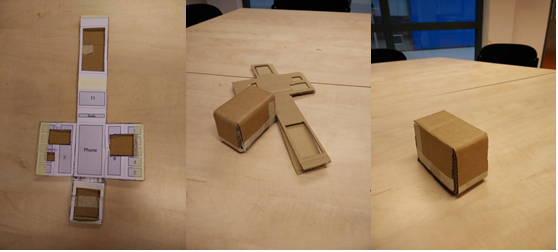
\includegraphics[width=0.8\textwidth]{resources/BoxPrototype1}
		\caption{Prototype of the first packaging redesign}
		\label{fig:Prototype of box design 1}
	\end{figure}
	
	Since the first design was discarded after creating the prototype, a second design originated. It was decided to maintain a stiff casing structure as is seen in most phone packaging designs, and implement a tray system. Instead of having the repair mat fold out of the box, different trays (coined as ``layers'') with appropriate slots were designed. This can better be seen in figure \ref{fig:Box design 2}. The layers are provided with a lip, which serves as a handle to remove it from the main box.
	
	\begin{figure}[H]
		\centering
		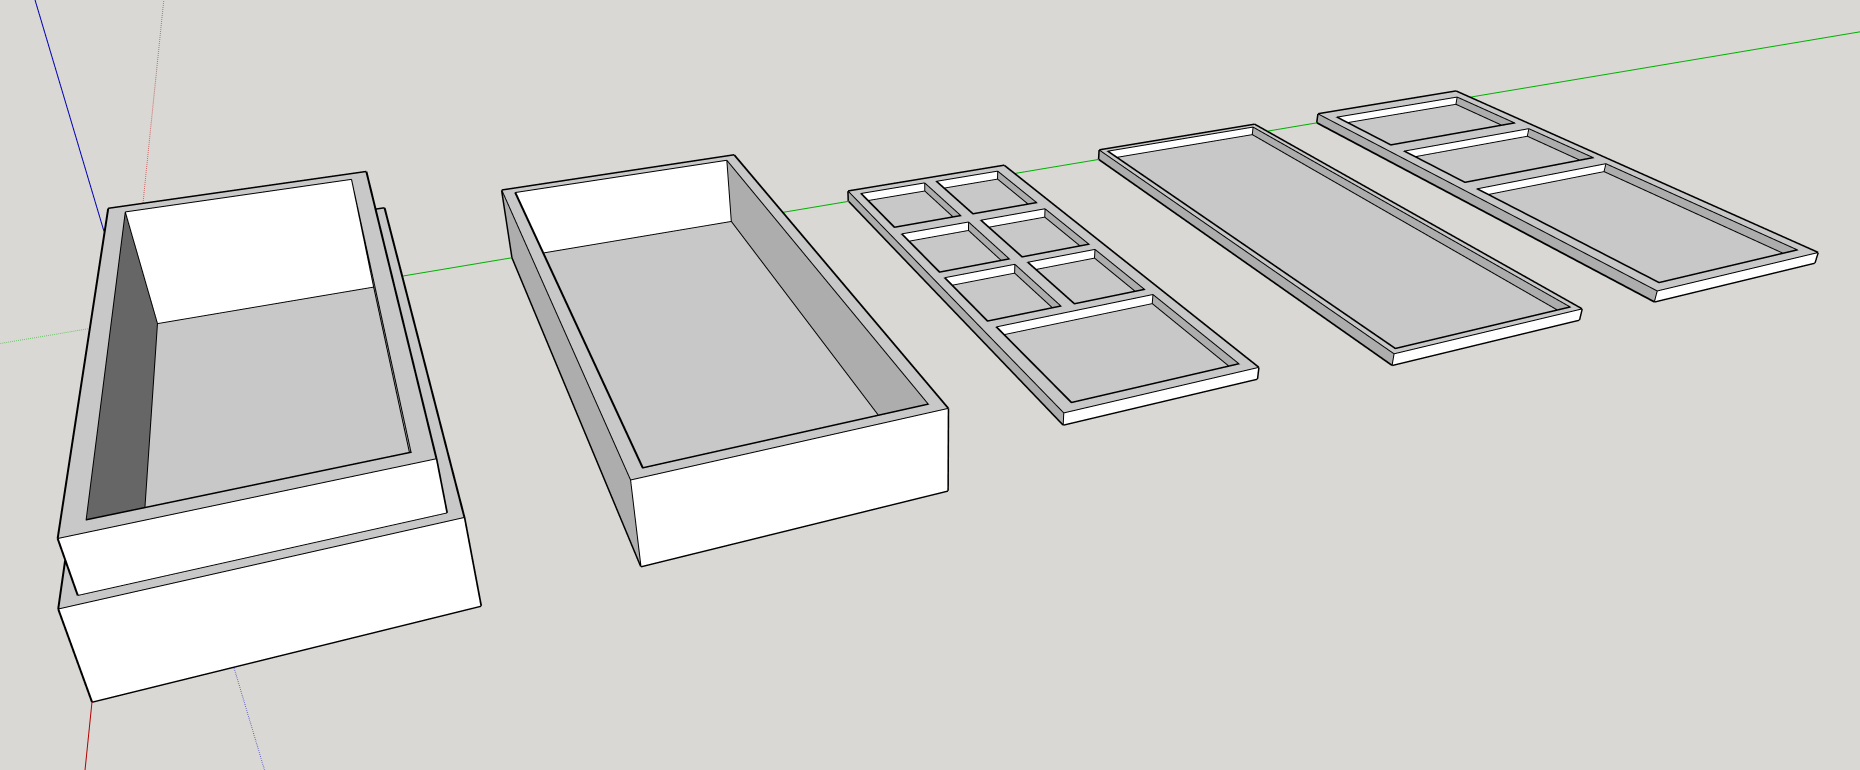
\includegraphics[width=0.8\textwidth]{resources/BoxDesign2}
		\caption{The second re-design of the Fairphone 2 packaging}
		\label{fig:Box design 2}
	\end{figure}
	
	Before prototyping this design, better quality low impact materials were acquired from the architecture faculty. Using these materials the new prototype was created. The result can be seen in figure \ref{fig:Prototype of box design 2}.
	
	\begin{figure}[H]
		\centering
		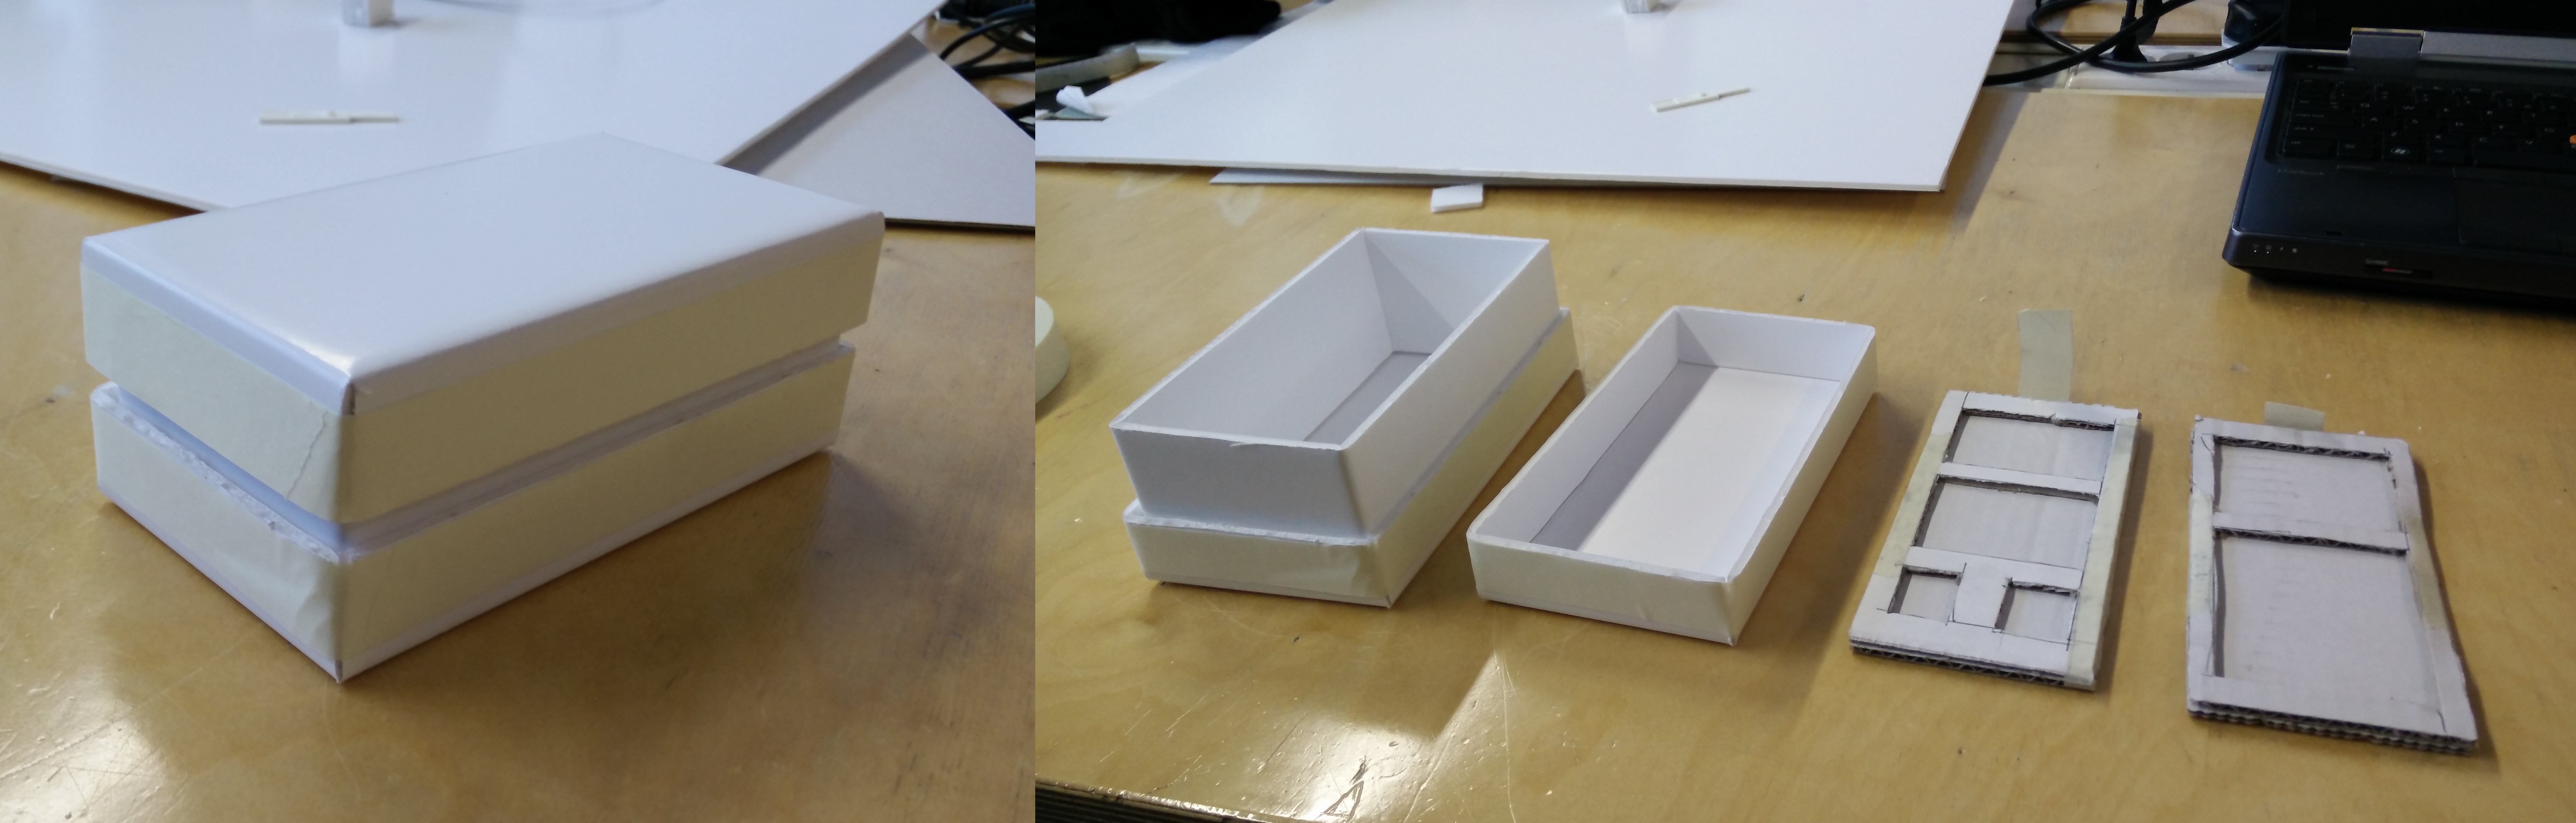
\includegraphics[width=0.8\textwidth]{resources/BoxPrototype21}
		\caption{Prototype of the first packaging redesign}
		\label{fig:Prototype of box design 2}
	\end{figure}
	
	Since the prototype served its function well, aesthetics were taken into consideration. Plain white revealed to be boring, and made it look fragile. In fact, it looked like it was made of simple paper. To make the packaging appear more elaborated and stronger, some cork details were added to the prototype to make it look and feel fairer as can be seen in figure \ref{fig:Prototype of box design 2 with cork details}.
	
	\begin{figure}[H]
		\centering
		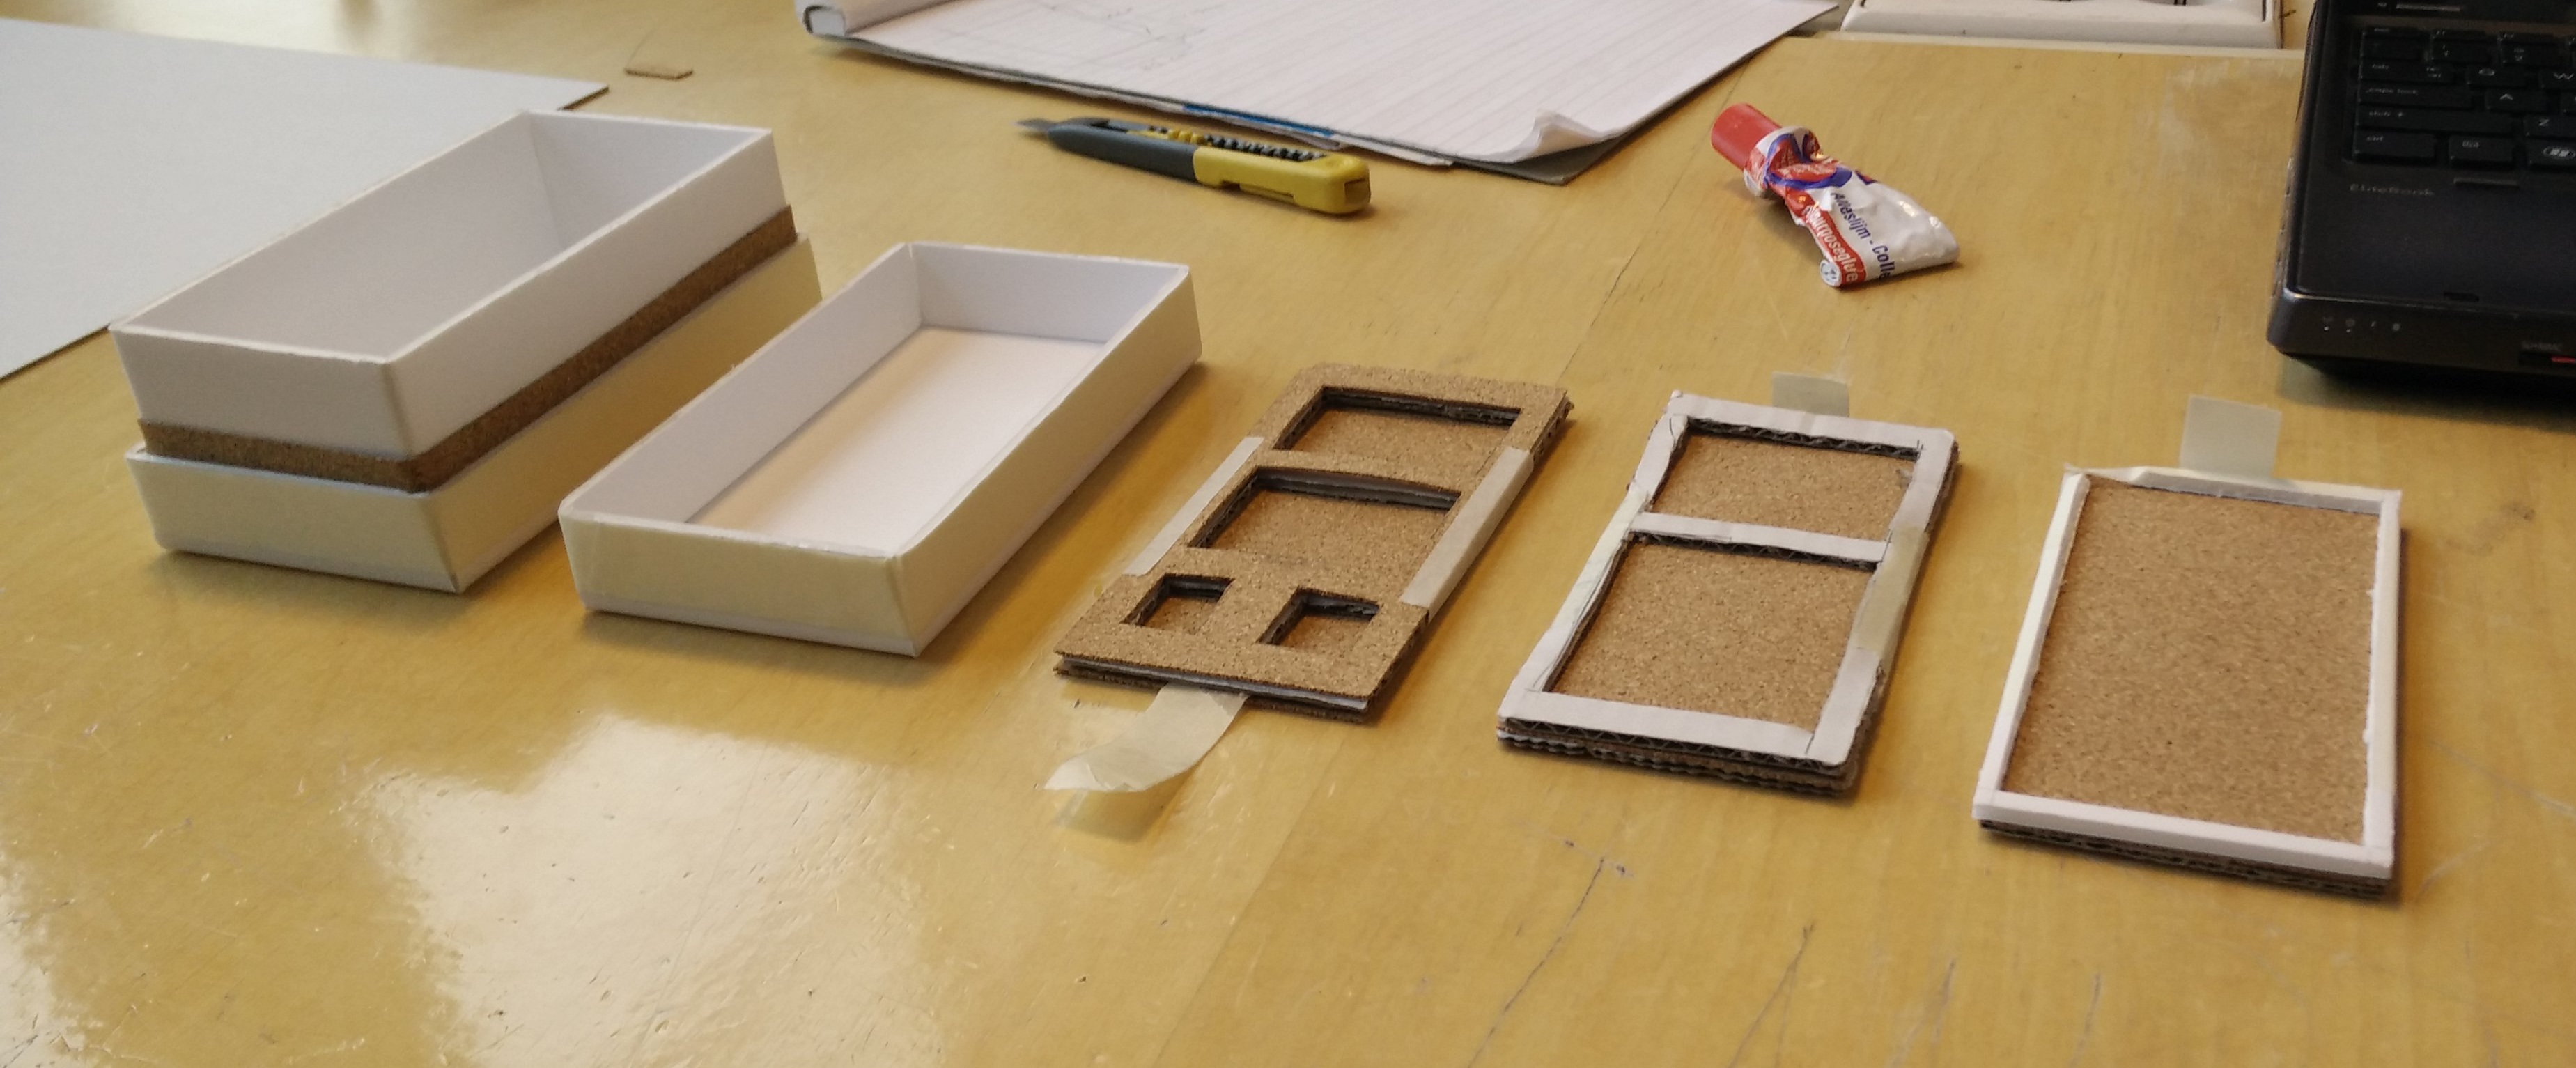
\includegraphics[width=0.8\textwidth]{resources/BoxPrototype22}
		\caption{Prototype of the second packaging redesign with cork details}
		\label{fig:Prototype of box design 2 with cork details}
	\end{figure}
	
	Even tough the second version of the second design was appreciated by the team, it was decided to make the layers entirely out of cork. This choice was made because cork is a lower grade material, and is strong enough to serve as a repair mat. This enhances the ``fair experience'' Fairphone so much strives for. This final prototype is also the one that will be used for the user testing of the product.
	
	\begin{figure}[H]
		\centering
		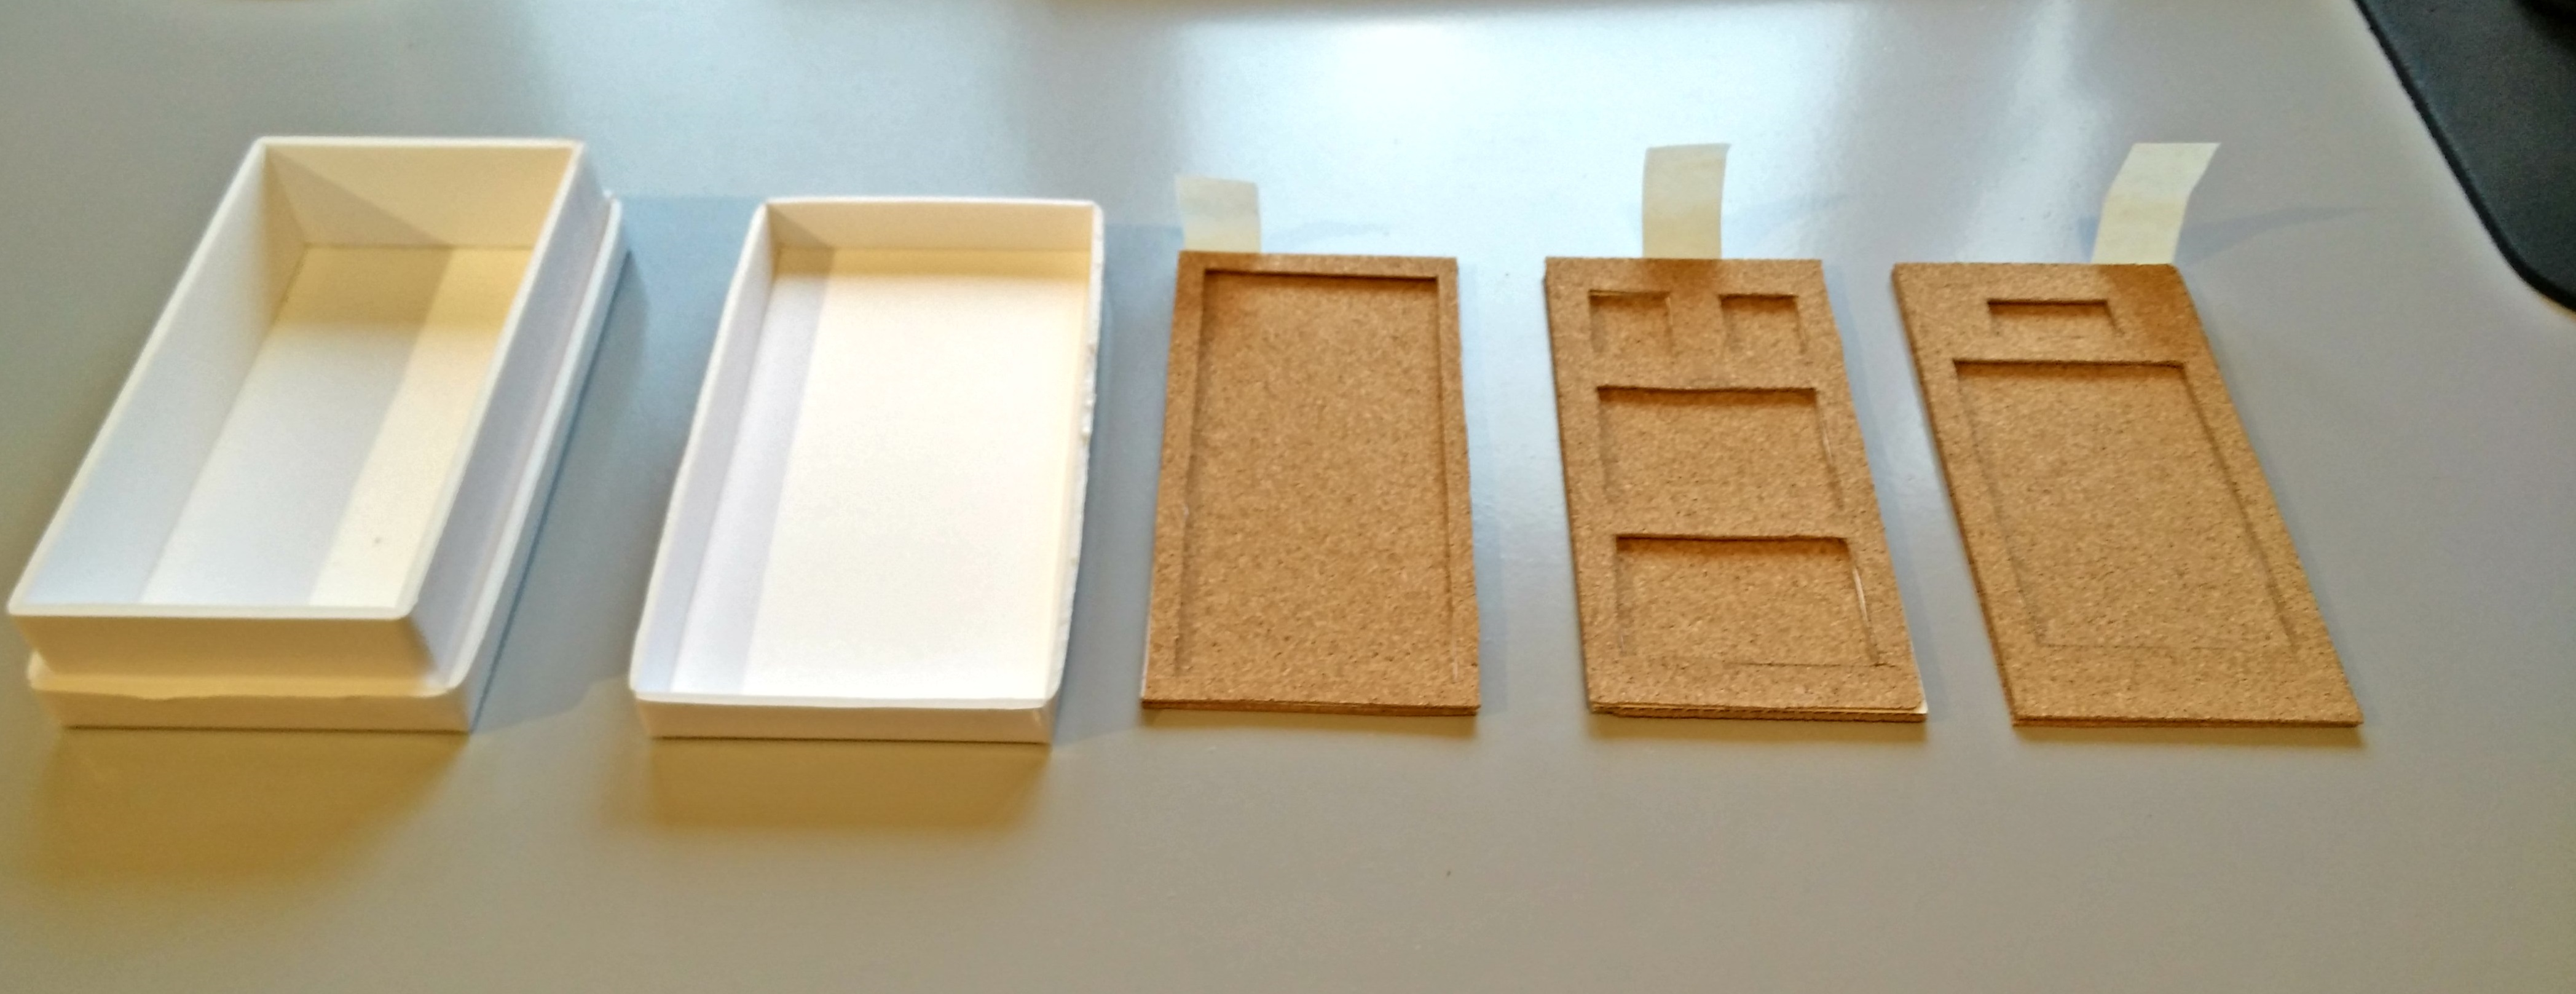
\includegraphics[width=0.8\textwidth]{resources/BoxPrototype23}
		\caption{Prototype of the second packaging redesign with full cork layers}
		\label{fig:Prototype of box design 2 with full cork exterior}
	\end{figure}  

	\subimport{user-testing/}{user-testing.tex}
	\subimport{feedback/}{feedback.tex}
	\subimport{improvements/}{improvements.tex}
\end{document}